\documentclass[paper=a4, fontsize=11pt]{scrartcl} % A4 paper and 11pt font size

\usepackage[utf8]{inputenc} % Use 8-bit encoding that has 256 glyphs
\usepackage{fourier} % Use the Adobe Utopia font for the document - comment thi
\usepackage[spanish]{babel} % English language/hyphenation
\usepackage{amsmath,amsfonts,amsthm} % Math packages
\usepackage{fixltx2e}
\usepackage{graphicx}


\usepackage{lipsum} % Used for inserting dummy 'Lorem ipsum' text into the temp

\usepackage{sectsty} % Allows customizing section commands
\allsectionsfont{\centering \normalfont\scshape} % Make all sections centered,

\usepackage{fancyhdr} % Custom headers and footers
\pagestyle{fancyplain} % Makes all pages in the document conform to the custom
\fancyhead{} % No page header - if you want one, create it in the same way as t
\fancyfoot[L]{} % Empty left footer
\fancyfoot[C]{} % Empty center footer
\fancyfoot[R]{\thepage} % Page numbering for right footer
\renewcommand{\headrulewidth}{0pt} % Remove header underlines
\renewcommand{\footrulewidth}{0pt} % Remove footer underlines
\setlength{\headheight}{13.6pt} % Customize the height of the header

\numberwithin{equation}{section} % Number equations within sections (i.e. 1.1,
\numberwithin{figure}{section} % Number figures within sections (i.e. 1.1, 1.2,
\numberwithin{table}{section} % Number tables within sections (i.e. 1.1, 1.2, 2

\setlength\parindent{0pt} % Removes all indentation from paragraphs - comment t

%------------------------------------------------------------------------------
%	TITLE SECTION
%------------------------------------------------------------------------------

\newcommand{\horrule}[1]{\rule{\linewidth}{#1}} % Create horizontal rule comman

\title{
\normalfont \normalsize
\textsc{Universidad EAFIT, } \\ [25pt] % Your university, sch
\horrule{0.5pt} \\[0.4cm] % Thin top horizontal rule
\huge Introducción a sistemas CAD/CAM \\ % The assignment title
\horrule{2pt} \\[0.5cm] % Thick bottom horizontal rule
}

\author{Santiago Hincapie} % Your name

\date{\normalsize\today} % Today's date or a custom date

\begin{document}

\maketitle
\section{Conceptos basicos}
\subsection{Funciones}
\subsubsection{Producto cartesiano}
El \textit{producto cartesiano} de dos conjuntos es una operación, que resulta
en otro conjunto, cuyos elemenentos son todos los pares ordenados que pueden
formarse de formar que el primer elemento del par ordenado perteneza al primer
onjunto y el segundo elemento pertenezca al segundo conjunto.\\

Mas formalmente el producto cartesiano de $A$ y $B$ es el conjunto $A \times B$
cuyos elementos son los pares ordenados $(a, b)$ donde $a$ es un elemento de $A$
y $b$ un elemento de $B$.

\[A \times B = \{(a, b): a \in A\ \&\ b \in B\}\]

\subsubsection{Relaciones}
Una \textit{relacion} $\mathcal{R}$, entre los conjuntos $A, B$ es un subconjunto
propio del producto cartesiano $A \times B$, en el cual se cumple cierta propiedad
$\mathcal{P}(a, b)$, de forma que $(a, b) \in A \times B$, es decir

\[\mathcal{R} = \{(a, b) \in A \times B\ |\ \mathcal{P}(a, b)\}\]

\subsubsection{Funcion}
Una \textit{funcion} $f : A \to B$ es un tipo muy especial de relacion, en la cual,
no existen dos pares distintos con la misma primera componente, es decir:
\[\text{si } (a, b) \in f(A)\ \land\ (a, c) \in f(A) \implies\ b = c\]

\subsubsection{Propiedades de las funciones}
\paragraph{Inyectiva}
Una funcion $f: A \to B$ es inyectiva si a elementos distintos del conjunto $A$ les
corresponde elemenentos distintos en el conjunto $B$
Mas formalmente una funcion $f: A \to B$ se dice que es inyectiva si
\[\forall_{a_1, a_2} \in A, a_1 \neq a_2 \implies f(a_1) \neq f(a_2)\]

Por ejemplo, la funcion $f : \mathbb{R} \to \mathbb{R}$, dada por $f(x) = x^2$ no es
inyectiva, pues el valor $1$ puede obtenerse de $f(1)$ o $f(-1)$. Pero si por otro
lado, se restringe el dominio a los reales positivos, creando una nueva funcion
$g: \mathbb{R}^+ \to \mathbb{R}^+$, dada por $g(x) = x^2$, esta nueva funcion si es
inyectiva.

\paragraph{Sobreyectiva}
Una funcion $f : A \to B$ es sobreyectiva si a cada elemento $b \in B$ existe al menos
un elemento $a \in A$ tal que $f(a) = b$. Asi por ejemplo, la funcion
$f : \mathbb{R} \to \mathbb{R}$, dada por $f(x) = |x|$ no es sobreyectiva pues en
particular no existe una preimagen para $x = -1 \in \mathbb{R}$, ahora, si se restringe
la el conjunto de llegada (AKA codominio) a los reales positivos, generando una nueva
funcion $g : \mathbb{R} \to \mathbb{R}^+$, dada por $g(x) = x^2$, esta nueva funcion es
sobreyectiva\\
Es importante notar que es facil construir una funcion que cumpla la condicion de
sobreyectividad, pues normalmente se posee control sobre los conjuntos de partida y
llegada.

\paragraph{Biyectiva}
Una funcion es biyectiva si es al mismo tiempo inyectiva y sobreyectiva; Es decir,
si todos los elementos del conjunto de salida tienen una imagen distinta en el
conjunto de llegada, y a cada elemento del conjunto de llegada le corresponde
un elemento del conjunto de salida.
Las funciones biyectivas son particularmente interesante pues si $f : A \to B$ es
biyectiva, existe una funcion $f^{-1} : B \to A$ tal que si $a \in A\ \land b \in B$
entonces $f(x) = y \implies f^{-1}(y) = x$.
Otra implicacion curiosa (y no muy importante para el curso) es que si 2 conjuntos
poseen la misma cardinalidad (el mismo numero de elementos) existe una biyeccion
entre ellos, esto ademas de tener una gran importancia matematica, trae una implicacion
real bastante interesante, cuando se enumera o se cuenta cualquier conjunto de cosas,
realmente lo que se está haciendo es establecer una biyeccion entre un subconjunto de
los numeros naturales y el conjunto de cosas que se esta numerando.

\subsection{Grupos}
\subsubsection{Operador binario}
Un operador binario $\odot$ es simplemente una funcion que recibe dos parametros
(operantes) $\odot(a, b) = a \odot b$.
\subsubsection{Grupo}
Un conjunto $G$ equipado con un operador binario $\odot : A \times A \to A$. $(G, \odot)$ es un
grupo si cumple las siguientes propiedades:
\begin{enumerate}
\item \textbf{Clausura} $\forall_{x, y} \in G \implies x \odot y \in G$ Esto quiere decir que
  al operar   cualquier par de elementos del conjunto $G$ utilizando el operador
  $\odot$ el resultado tambien es un elemento de $G$.
\item \textbf{Existencia de elemento neutro} $\exists_e \in G$ tal que $\forall_x \in G, x \odot e = e \odot x = x$
  Esto quiere decir que entre todos los elementos de $G$ debe existir alguno que
  ``no haga   nada al operarse'' con los otros elementos del grupo, ``el 0 de
  $G$''.
\item \textbf{Existencia de el elemento inverso} $\forall_x \in G \exists_{x^{-1}} \in G$ tal que
  $x \odot x^{-1} = x^{-1} \odot x = e$. Esto quiere decir que si yo seleciono un elemento de $G$
  \textbf{debe} existir otro que lo ``anule''.
\item \textbf{Asociatividad} $\forall_{x, y, z} \in G \implies x \odot y \odot z = (x \odot y) \odot z = x \odot (y \odot z)$
  La intuicion detras de esta propiedad es bastante simple, que al operar $3$
  valores bajo el operador $\odot$ pueda agruparlos de la forma que desee y esto no
  cambiará el resultado.
\end{enumerate}

\subsection{Grupo linear general}
\subsubsection{Grupo lineal general (GL)}
El grupo $GL(n) = (M_n, \cdot)$ esta formado por el conjunto de todas las matrices
reales de tamaño $n \times n$ invertibles (AKA $M_n$), equipado con el producto
estandar de matrices $(\cdot)$

\subsubsection{Grupo lineal postivo}
El grupo $GL^+(n) = (M_n^+, \cdot)$ esta formado por el subconjunto de todas las
matrices reales de tamaño $n \times n$, $A$, tales que $\det(A) > 0$ (AKA $M_n^+$),
equipado con el producto estandar de matrices $(\cdot)$

\subsubsection{Grupo ortogonal}
El grupo $O(n)$ es el subconjunto de $GL(n)$ formado por las matrices $A$ tales
que $A \cdot A^T = I$, es posible demostrar que $\det(A) = \pm 1$

\subsubsection{Grupo ortogonal especial}
El grupo $SO(n)$ es el subconjunto de $O(n)$ formado por las matrices $A$ tales
que $\det(A) = +1$.\\

La figura\ref{fig:o} posee un resumen de esta informacion
\begin{figure}[!ht]
  \centering
  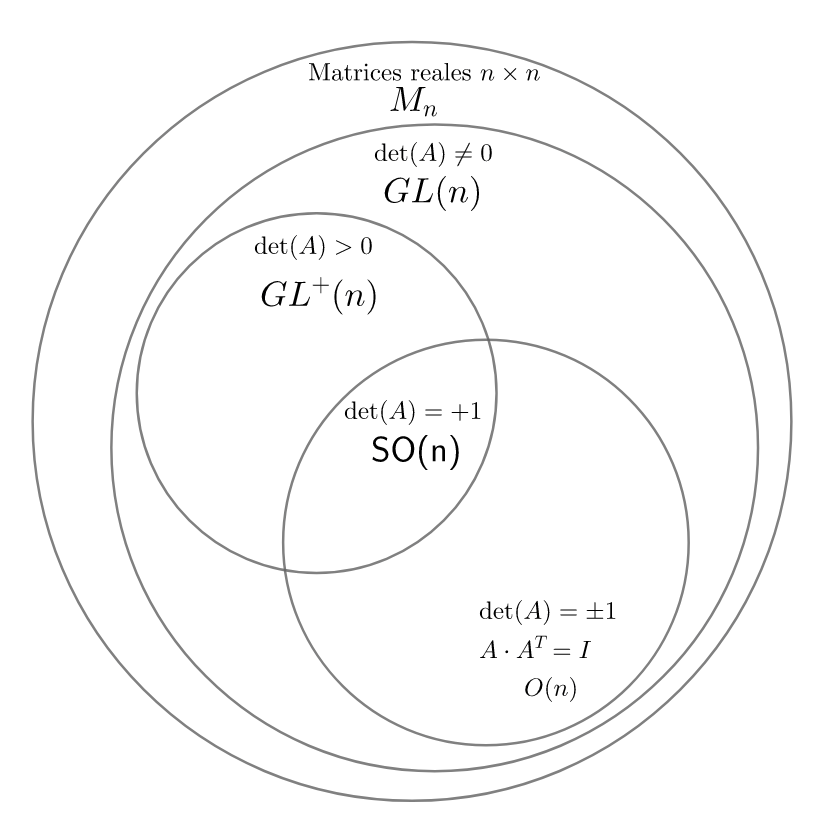
\includegraphics[scale=0.3]{rsc/set}
  \caption{Grupo ortogonal y ortogonal especial}\label{fig:o}
\end{figure}

\subsection{Transformaciones}
Una transformacio $f : A \to B$ es una funcion, con $A, B \subset \mathbb{R}^n$ que cumple:
\begin{enumerate}
  \item $f$ es bijectiva
  \item las derivadas parciales de cualquier orden de $f$ son continuas.
  \item $\det(J_f) \neq 0$, es decir, el determinante de la matrix jacobiana
    es diferente de $0$ para cualquier valor de la funcion $f$
\end{enumerate}
\[J_f =
\begin{pmatrix}
  \dfrac{\partial f_1}{\partial x_1} & \cdots & \dfrac{\partial f_1}{\partial x_n} \\
           \vdots           & \ddots &         \vdots           \\
  \dfrac{\partial f_n}{\partial x_1} & \cdots & \dfrac{\partial f_n}{\partial x_n}  \\
\end{pmatrix}\]
\subsubsection{Transformacion lineal}
una transformacion lineal $f : \mathbb{R}^n \to \mathbb{R}^n$ tiene la forma
$f(p) = A \cdot p$ donde $A \in GL(n), p \in \mathbb{R}^n$ y $\cdot$ es el producto
estandar de matrices.

\subsubsection{Transformacion afín}
Si $f : \mathbb{R}^n \to \mathbb{R}^n$ transforma cualquier linea recta en otra
linea recta, luego se dice que $f$ es una transformacion afin. Una
transformacion afin tiene la forma $f_{A, T}(p) = A \cdot p + T$, donde
$A \in GL(n); T, p \in \mathbb{R}^n$ y $\cdot$ es el producto estandar de matrices.

La figura\ref{fig:t} posee un resumen de esta informacion
\begin{figure}[!ht]
  \centering
  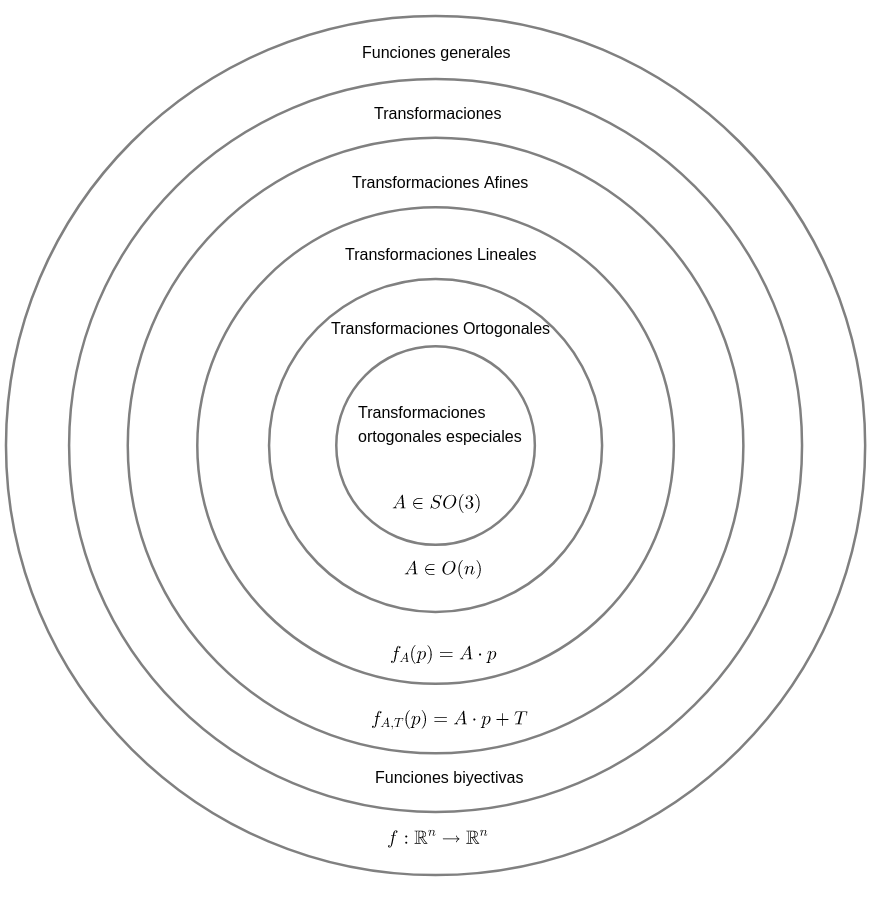
\includegraphics[scale=0.3]{rsc/trans}
  \caption{Grupo ortogonal y ortogonal especial}\label{fig:t}
\end{figure}

%\section{invarianza}

\end{document}
